\chapter{Design}\label{ch:design}

This section discusses the design of the system. The first part explains query
spawning and execution, the second part describes how data stream can be shared
between queries.

\section{Overall Architecture}

Our system consists of multiple components which are briefly described in this
paragraph. A dataflow program submitted to run as part of the system is
called a \emph{query}. Following Timely's terminology, the execution of a query
is done by a group of \emph{worker} threads. Each worker manages the scheduling and
notification of the nodes that are part instance of the dataflow graph.

A query is executed by one or more \emph{executors}. Each executor selected to
execute a query will fetch and invoke the query binary, ultimately spawning the
worker threads.

All these components are managed by a central process called the
\emph{coordinator}. To achieve this, the coordinator hosts the \emph{catalog}, a
datastructure which contains all information about the available executors, the
running queries and their workers.

\begin{figure}[ht]
  \centering
    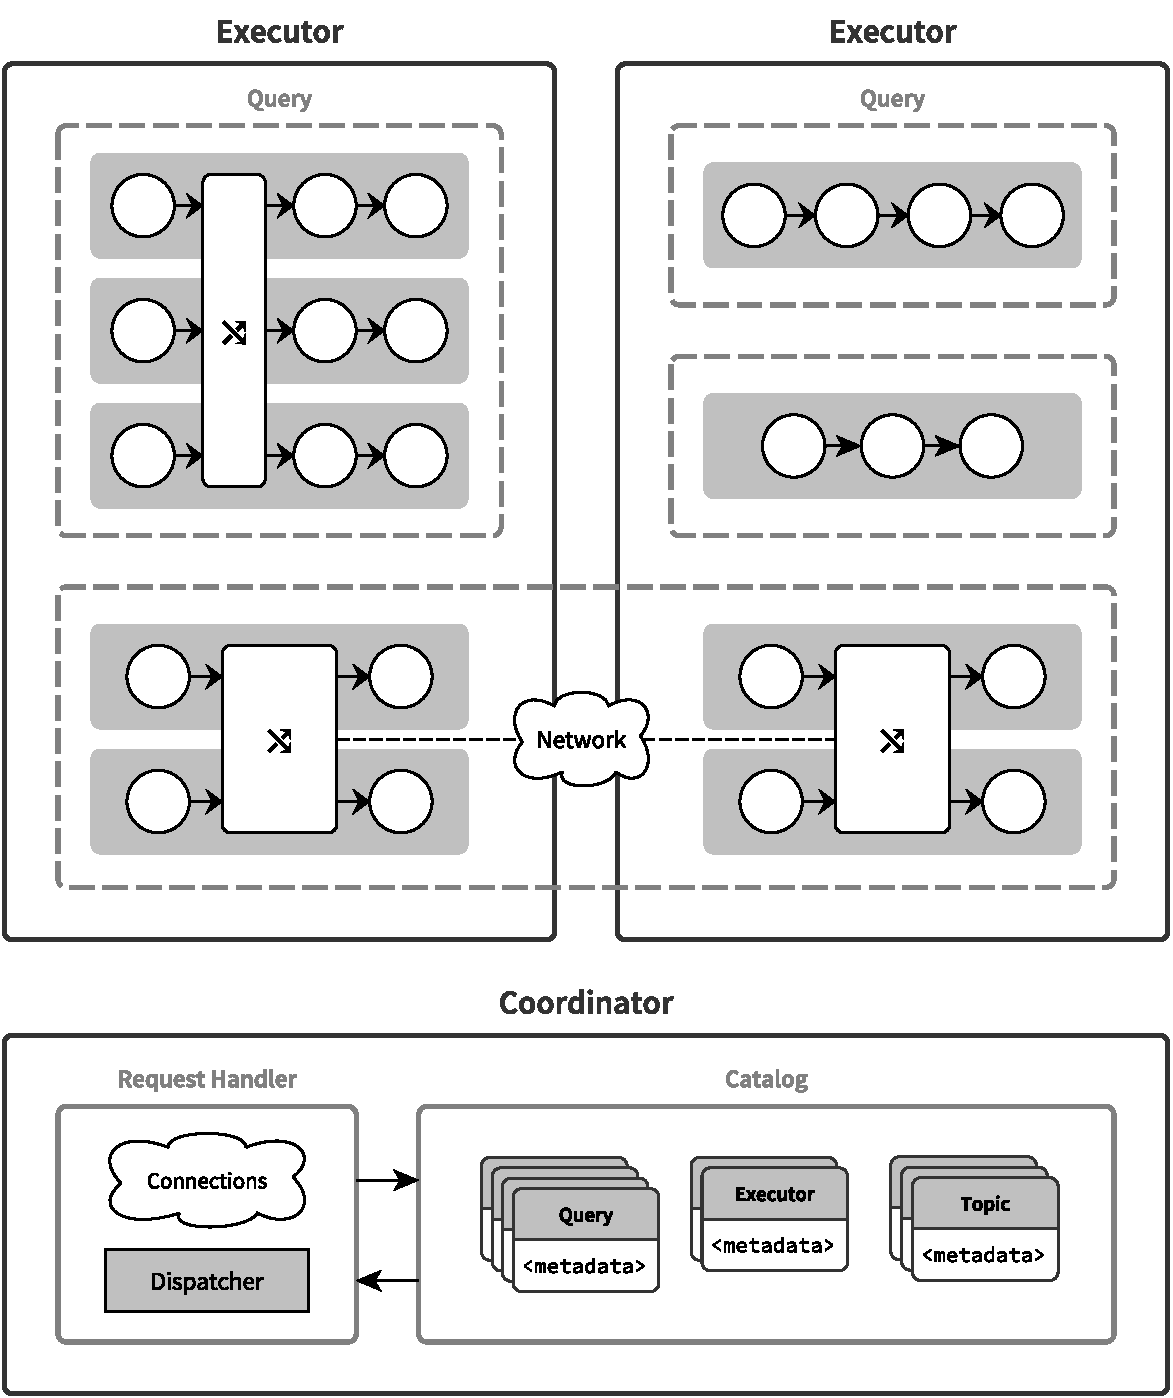
\includegraphics[width=1\textwidth]{figures/components}
  \caption[System architecture.]{ Queries (dashed boxes) consist of one or
  more worker threads (rounded grey boxes) driving the dataflow computation.
  A query might spawn over multiple executors, make use of the network for message exchanges
  between the workers of a query.\\
  The coordinator maintains a connection to every  executor and every query process.
  The state of the whole system is stored in the catalog.}
  \label{fig:components}
\end{figure}

\section{Queries}

A query is a Timely Dataflow program managed and executed by our system. Like
standalone Timely Dataflow programs, queries are written in Rust by using the
Timely Dataflow library: The dataflow graph is constructed by connecting
Timely's operators (vertices) to stream objects (edges).

In order for a Timely Dataflow program to become a runnable query on the system,
it needs to register its computational logic with with our system library instead of
using Timely Dataflow's initialization function. This
\lstinline{timely_query::execute} function not only performs the initialization
for the query, it also provides additional methods to interact with the catalog.

\begin{lstlisting}[caption={[Example query.]Example query which creates a stream of integers,
filters out all odd numbers and then prints the rest.}]
extern crate timely;
extern crate timely_query;

use timely::dataflow::Scope;
use timely::dataflow::operators::{Filter, Inspect, ToStream};

fn main() {
    timely_query::execute(|root, catalog| {
        root.scoped::<u32, _, _>(|scope| {
            (0..100).to_stream(scope)
                .filter(|x| x % 2 == 0)
                .inspect(|x| println!("hello {:?}", x));
        });
    }).unwrap();
}
\end{lstlisting}


TODO This is the description of a query from the user perspective. How does the
coordinator see it?

\subsection{Submission}

The compilation of a query's source code into a runnable binary is done
at the client side. This allows the user to link against arbitrary
libraries which they might use in their query program. 

\section{Execution}



\section{Communication paradigm}

Pubsub

\section{Execution model}
